\documentclass{article}
\usepackage[margin=1in]{geometry}
\usepackage{microtype}
\usepackage{setspace}
\usepackage{amsmath}
\usepackage{parskip}
\usepackage{amssymb}
\usepackage{graphicx}

\graphicspath{{../public/}}

\parskip=4ex
\date{}
\author{}

\title{12.3 Double Integrals in Polar Coordinates}

\begin{document}
  \maketitle
  \textbf{Introduction}\\
  Suppouse we want to evaluate a double integral $ \iint_R f(x,y)~dA $, where $ R $ is one of the regions shown below. In either case the description of $ R $ in a traditonal coordiante system is complicated. However, $ R $ is easily described by using polar coordinates.

  \begin{center}
    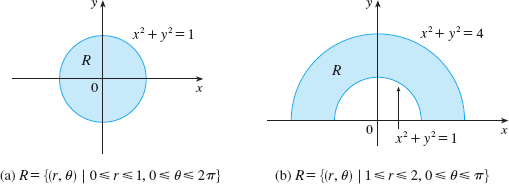
\includegraphics[width=12cm]{12_3_1}
  \end{center}

  Recall from the figure below that the polar coordinates $ (r,\theta) $ of a point are related to the rectangular coordinates $ (x,y) $ by the equations
  \[
    \boxed{r^{2}=x^{2}+y^{2} \qquad x=r\cos{\theta} \qquad y=r\sin{\theta}}
  \]

  \begin{center}
    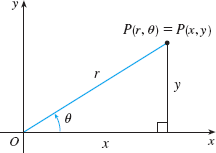
\includegraphics[width=6cm]{12_3_2}
  \end{center}
 
  The regions in the first figure are special cases of a polar rectangle
  \[
    R=\{ (r,\theta) | a \le r \le, \alpha \le \theta \le \beta \}
  \]
  shown in the figure below.

  \begin{center}
    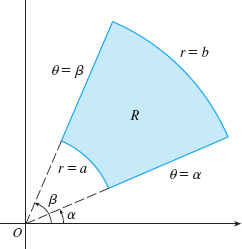
\includegraphics[width=5cm]{12_3_3}
    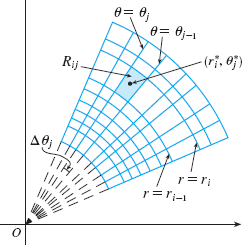
\includegraphics[width=5cm]{12_3_4}
  \end{center}

  The area of $ R_ij $ is
  \[
    r^{*}_i \Delta r_i \Delta \theta_j
  \]
  

  The rectangular coordinates of the center of $ R_{ij} $ are $ (r^{*}_i\cos{\theta}^{*}_j), r^{*}_i\sin{\theta}^{*}_j $, so a typical Riemann sum is
  \[
   \sum^{m}_{i=1} \sum^{n}_{j=1} f(r^{*}_i \cos{\theta}^{*}_j,r^{*}_i \sin{\theta}^{*}_j) \Delta A_{ij} = \sum^{m}_{i=1} \sum^{n}_{j=1} f(r^{*}_i \cos{\theta}^{*}_j,r^{*}_i \sin{\theta}^{*}_j) r^{*}_i \Delta r_i \Delta \theta_j
  \]

  If we write $ g(r,\theta)= r f(r\cos{\theta},r\sin{\theta}) $, the Riemann sum becomes
  \[
    \sum^{m}_{i=1}\sum^{n}_{j=1} g(r^{*}_i, \theta^{*}_j)   
  \]

  Which is a Riemann sum for the double integral
  \[
    \int^{\beta}_{\alpha} \int^{b}_{a} g(r,\theta) ~ dr d\theta
  \]

  Which is also
  \[
    \int^{\beta}_{\alpha} \int^{b}_{a} f(r\cos{\theta},r\sin{\theta})r ~drd\theta 
  \]

  \textbf{Ex 1}\\
  Evaluate $ \iint_R 3x+4y^{2}~dA $, where $ R $ is the region in the  upper halfplane bounded by the circles $ x^{2}+y^{2}=1 ~\&~ x^{2}+y^{2}=4 $

  The region $ R $ can be described as
  \[
    R=\{ (x,y) | y \ge 0, 1 \le x^{2}+y^{2} \le 4 \}
  \]

  \begin{center}
    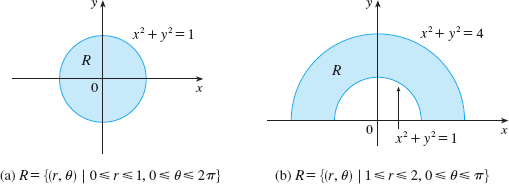
\includegraphics[width=10cm]{12_3_1}
  \end{center}

  $ R $ is the half right shown on the figure above (right side). In polar coordinates it is given by $ 1 \le r \le 2 ~\&~ 0 \le \theta \le \pi $.

  Therefore
  \[
    \begin{gathered}
    \iint_R 3x+4y^{2}~dA = \int^{\pi}_{0} \int^{2}_{1} 3(r\cos{\theta})+4(r^{2}\sin^{2}{\theta})r ~ dr d\theta\\
    \int^{\pi}_{0} \text{\huge{[}} \int^{2}_{1} 3r^{2}\cos{\theta}+4r^{3}\sin^{2}{\theta}~dr \text{\huge{]}} ~ d\theta\\
    \int^{\pi}_{0} \text{\huge{[}} r^{3}\cos{\theta}+r^{4}\sin^{2}{\theta} \text{\huge{]}}^{r=2}_{r=1}~d\theta\\
    \int^{\pi}_{0} 7\cos{\theta}+15\sin^{2}{\theta}~d\theta\\
    \int^{\pi}_{0} 7\cos{\theta}+\frac{15}{2}(1-\cos{2\theta})~d\theta\\
    7\sin{\theta}+\frac{15}{2}\theta-\frac{15}{4}\sin{2\theta} \bigg|^{\pi}_0=\boxed{\frac{15\pi}{2}}
    \end{gathered}
  \]

  \textbf{Ex 2}\\
  Find the volume of the solid bounded by the plane $ z=0 $ and the paraboloid $ z=1-x^{2}-y^{2} $.

  By setting $ z=0 $ in the equation $ z=1-x^{2}-y^{2} $, we get the equation $ x^{2}+y^{2}=1 $. Meaning that the plane intersects the circle $ x^{2}+y^{2}=1 $ formed by the paraboloid. The solid lies under the paraboloid and above the circular disk $ D $ given by $ x^{2}+y^{2} \le 1 $.

  In terms of polar coordinates $ D $ is given by $ 0 \le r \le 1 ~\&~ 0 \le \theta \le 2\pi $. Since $ 1-x^{2}-y^{2}=1 - r^{2} $, derived from the Pythagorean Theorem $ x^{2}+y^{2}=r^{2} $.

  \begin{center}
    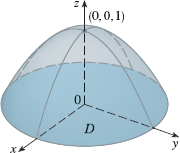
\includegraphics[width=4cm]{12_3_5}
  \end{center}

  \[
    \begin{gathered}
    V = \iint_D 1-x^{2}-y^{2}~dA = \int^{2\pi}_{0} \int^{1}_{0} (1-r^{2})r ~drd\theta\\
  \int^{2\pi}_{0} ~d\theta \int^{1}_{0} r-r^{3}~dr = 2\pi \text{\huge{[}} \frac{r^{2}}{2}-\frac{r^{4}}{4} \text{\huge{]}}^{1}_0=\boxed{\frac{\pi}{2}}
    \end{gathered}
  \]

  What has been done so far can be extended to more complicated region types shown in the figure below.
  
  \begin{center}
    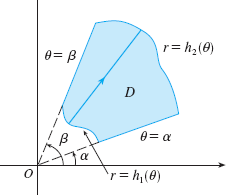
\includegraphics[width=6cm]{12_3_6}
  \end{center}

  \textbf{Theorem}\\
  If $ f $ is continuous on a polar region of the form
  \[
    D=\{ (r,\theta) | \alpha \le \theta \le \beta, h_1(\theta) \le r \le h_2(\theta) \}
  \]

  then
  \[
    \iint_D f(x,y)~dA = \int^{\beta}_{\alpha} \int^{h_2(\theta)}_{h_1(\theta)} f(r\cos{\theta},r\sin{\theta})r ~drd\theta 
  \]
  
  \textbf{Ex 3}\\
  Find the volume of the solid that lies under the parabolid $ z=x^{2}+y^{2} $, above the $ xy $ plane and inside the cylinder $ x^{2}+y^{2}=2x $.

  Since $ x=r\cos{\theta}, x^{2} +y^{2}=2x \to r^{2} =2x \to r^{2}=2r\cos{\theta} \to r=2\cos{\theta}$.
  \[
    D=\{ (r,\theta) | -\frac{\pi}{2}\le \theta, \frac{\pi}{2}, 0 \le r \le 2 \cos{\theta} \}
  \]
  
  Then we get
  \[
    \begin{gathered}
    V=\iint_D x^{2}+y^{2} = \int^{\frac{\pi}{2}}_{-\frac{\pi}{2}} \int^{2\cos{\theta}}_{0} r^{2}r ~ drd\theta = \int^{\frac{\pi}{2}}_{-\frac{\pi}{2}} \text{\huge{[}} \frac{r^{4}}{4} \text{\huge{]}}^{2\cos{\theta}}_0~d\theta\\
    4 \int^{\frac{\pi}{2}}_{-\frac{\pi}{2}} \cos^{4}{\theta}~d\theta=\boxed{\frac{3\pi}{2}}
    \end{gathered}
  \]
  
  
\end{document}
